% Requires \usepackage{graphicx}. Adjust the path for your manuscript.
% Caption matches configs/config.json; revise it for other experiments.
\begin{figure*}[t]
  \centering
  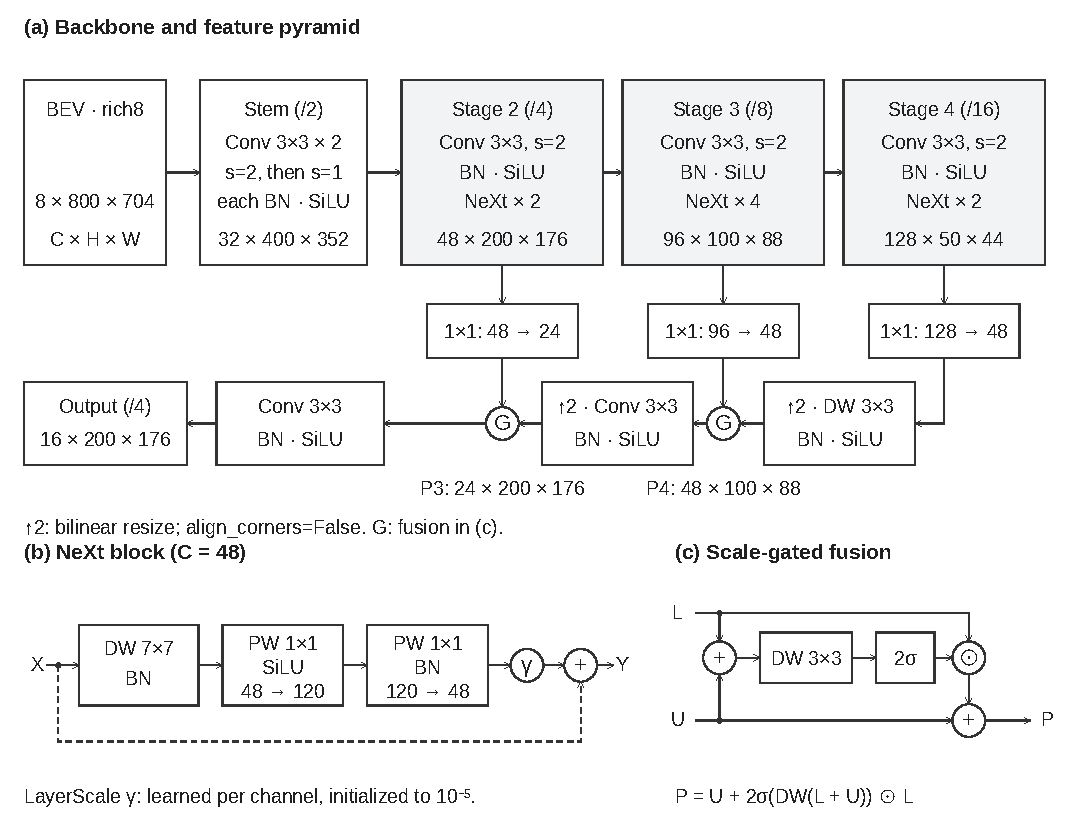
\includegraphics[width=\textwidth]{diagrams/paper_2d/backbone.pdf}
  \caption{Architecture of MobilePixorNeXt with a scale-gated feature pyramid.
  (a) The rich8 BEV input is encoded by a two-convolution stem and three stages
  with 2, 4, and 2 NeXt blocks, respectively. Lateral projections and top-down
  refinements produce a 16-channel feature map at stride 4. Tensor dimensions
  are shown as $C\times H\times W$, omitting the batch dimension.
  (b) A representative 48-channel block uses depthwise (DW) convolution,
  pointwise (PW) expansion to 120 channels, projection, and a residual connection
  with learned per-channel LayerScale $\gamma$, initialized to $10^{-5}$.
  (c) Fusion computes $P=U+2\sigma(\operatorname{DW}(L+U))\odot L$, where $L$
  is the lateral feature and $U$ is the resized and refined top-down feature.
  The gate convolution is initialized to zero, giving an initial gate of one.}
  \label{fig:mobilepixornext-backbone}
\end{figure*}
